\chapter{The sPHENIX Project}
\label{chap:project}

The sPHENIX detector is being realized via several projects that are
coordinated under a common project management structure.  There are
the elements of the original DOE Major Item of Equipment (MIE) --- the outer hadronic calorimeter (oHCal), the
central rapidity portion of electromagnetic calorimeter (EMCal)
covering $|\eta| < 0.85$, the time projection chamber (TPC), and their
associated readout electronics and services.  A silicon strip tracker
(INTT) is being provided by RIKEN.  Additional tungsten/scintillating
fiber blocks extending the coverage of the EMCal to $|\eta| < 1.1$ are
being provided by a consortium of collaborating institutions.
The inner longitudinal section of the hadronic calorimeter (iHCal) and
the silicon pixel vertex detector (MVTX) are being pursued as BNL
capital projects.  A quartz \v{C}erenkov minimum bias detector,
originally built by Hiroshima University for the PHENIX experiment, is
being re-purposed for use in sPHENIX.  There are also BNL funded
projects to upgrade the infrastructure at IP8, to operate the 1.5~T BaBar
superconducting solenoid, and to integrate and
install the sPHENIX detector into the IP8 area.  A labeled depiction of the
sPHENIX detector is shown in Figure~\ref{fig:sPHENIX}.

\section{Project timeline}
\label{sec:timeline}

The sPHENIX MIE received Critical Decision (CD)-1/3A approval in August 2018.  A memo from
DOE that same summer specified that projects below \$50M would no
longer be managed under DOE Order 413.3B, but would instead be managed
by the Laboratories, the details of which were to be worked out
between the National Laboratories and DOE.  The end result was that
sPHENIX would be working toward Project Decisions (PDs), to be
approved by the BNL Laboratory Director with DOE concurrence.  sPHENIX
received PD-2/3 approval in September 2019, and the most recent annual Cost \& Schedule Review in July 2020 was very positive.  The MIE has an early
completion date of November 2021 and a PD-4 date of December 2022.
The PD-4 goal is to provide a detector at RHIC ready to take 
commissioning data with collisions.

\section{Elements of the Project}
\label{sec:elements}

The full sPHENIX project consists of a large number of different
elements, some of which are a DOE major Item of Equipment (MIE) project,
others are part of an
upgrade to the infrastructure in Bldg. 1008, others are BNL capital
projects, and others are contributions from collaborating
institutions.  It is beyond the scope of this document to describe all
aspects of the project in great detail; instead we will focus on
the significant progress that has been made with detector elements
since the last NPP Program Advisory Committee meeting.

\subsection{MIE}

The MIE consists of six detector projects and management of the
MIE and related projects.
The detector systems are:

\begin{itemize}
    \item The compact (80 cm radius), ungated Time Projection Chamber (TPC), with GEM-based readout digitized via modified SAMPA ASICs, which were developed for the ALICE experiment
    \item The electromagnetic calorimeter, a tungsten-scintillating fiber
    SPACAL read out with solid state photomultiplier (SiPM's)
    \item The outer hadronic calorimeter, tilted steel plates with scintillating tiles
    interspersed in slots, also read out with SiPM's, which also doubles
    as the flux return of the 1.5 T superconducting solenoid
    \item Common electronics to read out both calorimeters consisting of
    shaper amplifiers on the detector which bring analog signals to 60 MHz waveform digitizers outside the solenoid
    \item Data acquisition designed to be capable of taking minimum bias
    Au+Au collisions at 15 kHz with greater than 90\% livetime, and minimum bias triggers for Au+Au collisions, and jet and photon triggers for p+p and p+A operation
    \item The Minimum Bias Detector (MBD), which consists of the refurbished PHENIX Beam-Beam Counter (BBC), read out and triggered with new electronics based on the digitizers designed for the calorimeters
\end{itemize}

All of the detector systems are under construction and the TPC and calorimeter prototypes have been tested in beam at Fermilab.

\begin{figure}[hbt!]
  \centering
  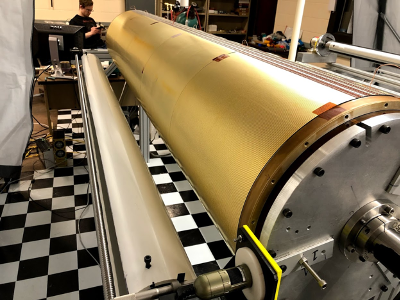
\includegraphics[width=0.49\linewidth]{innerfieldcage}
  \hfill
  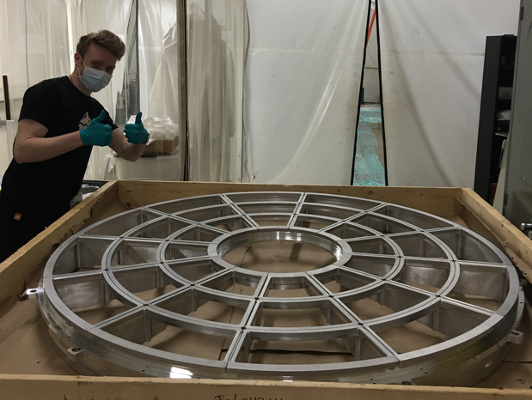
\includegraphics[width=0.49\linewidth]{wagonwheel}
  \caption{(left) The inner field cage of the TPC. A length of PVC
    sewer pipe, milled to a precise outer diameter, was used as an
    economical form upon which the field cage was built.  (right) One
    of the two TPC ``wagon wheels'' which supports the TPC field
    cages, the GEMs, the readout electronics and all the services.
    The wheels are each milled from a single billet of aluminum
    improving the gas tightness of the TPC by eliminating a large
    number of seams.}
  \label{fig:wagonwheel}
\end{figure}

\begin{figure}[hbt!]
  \centering
  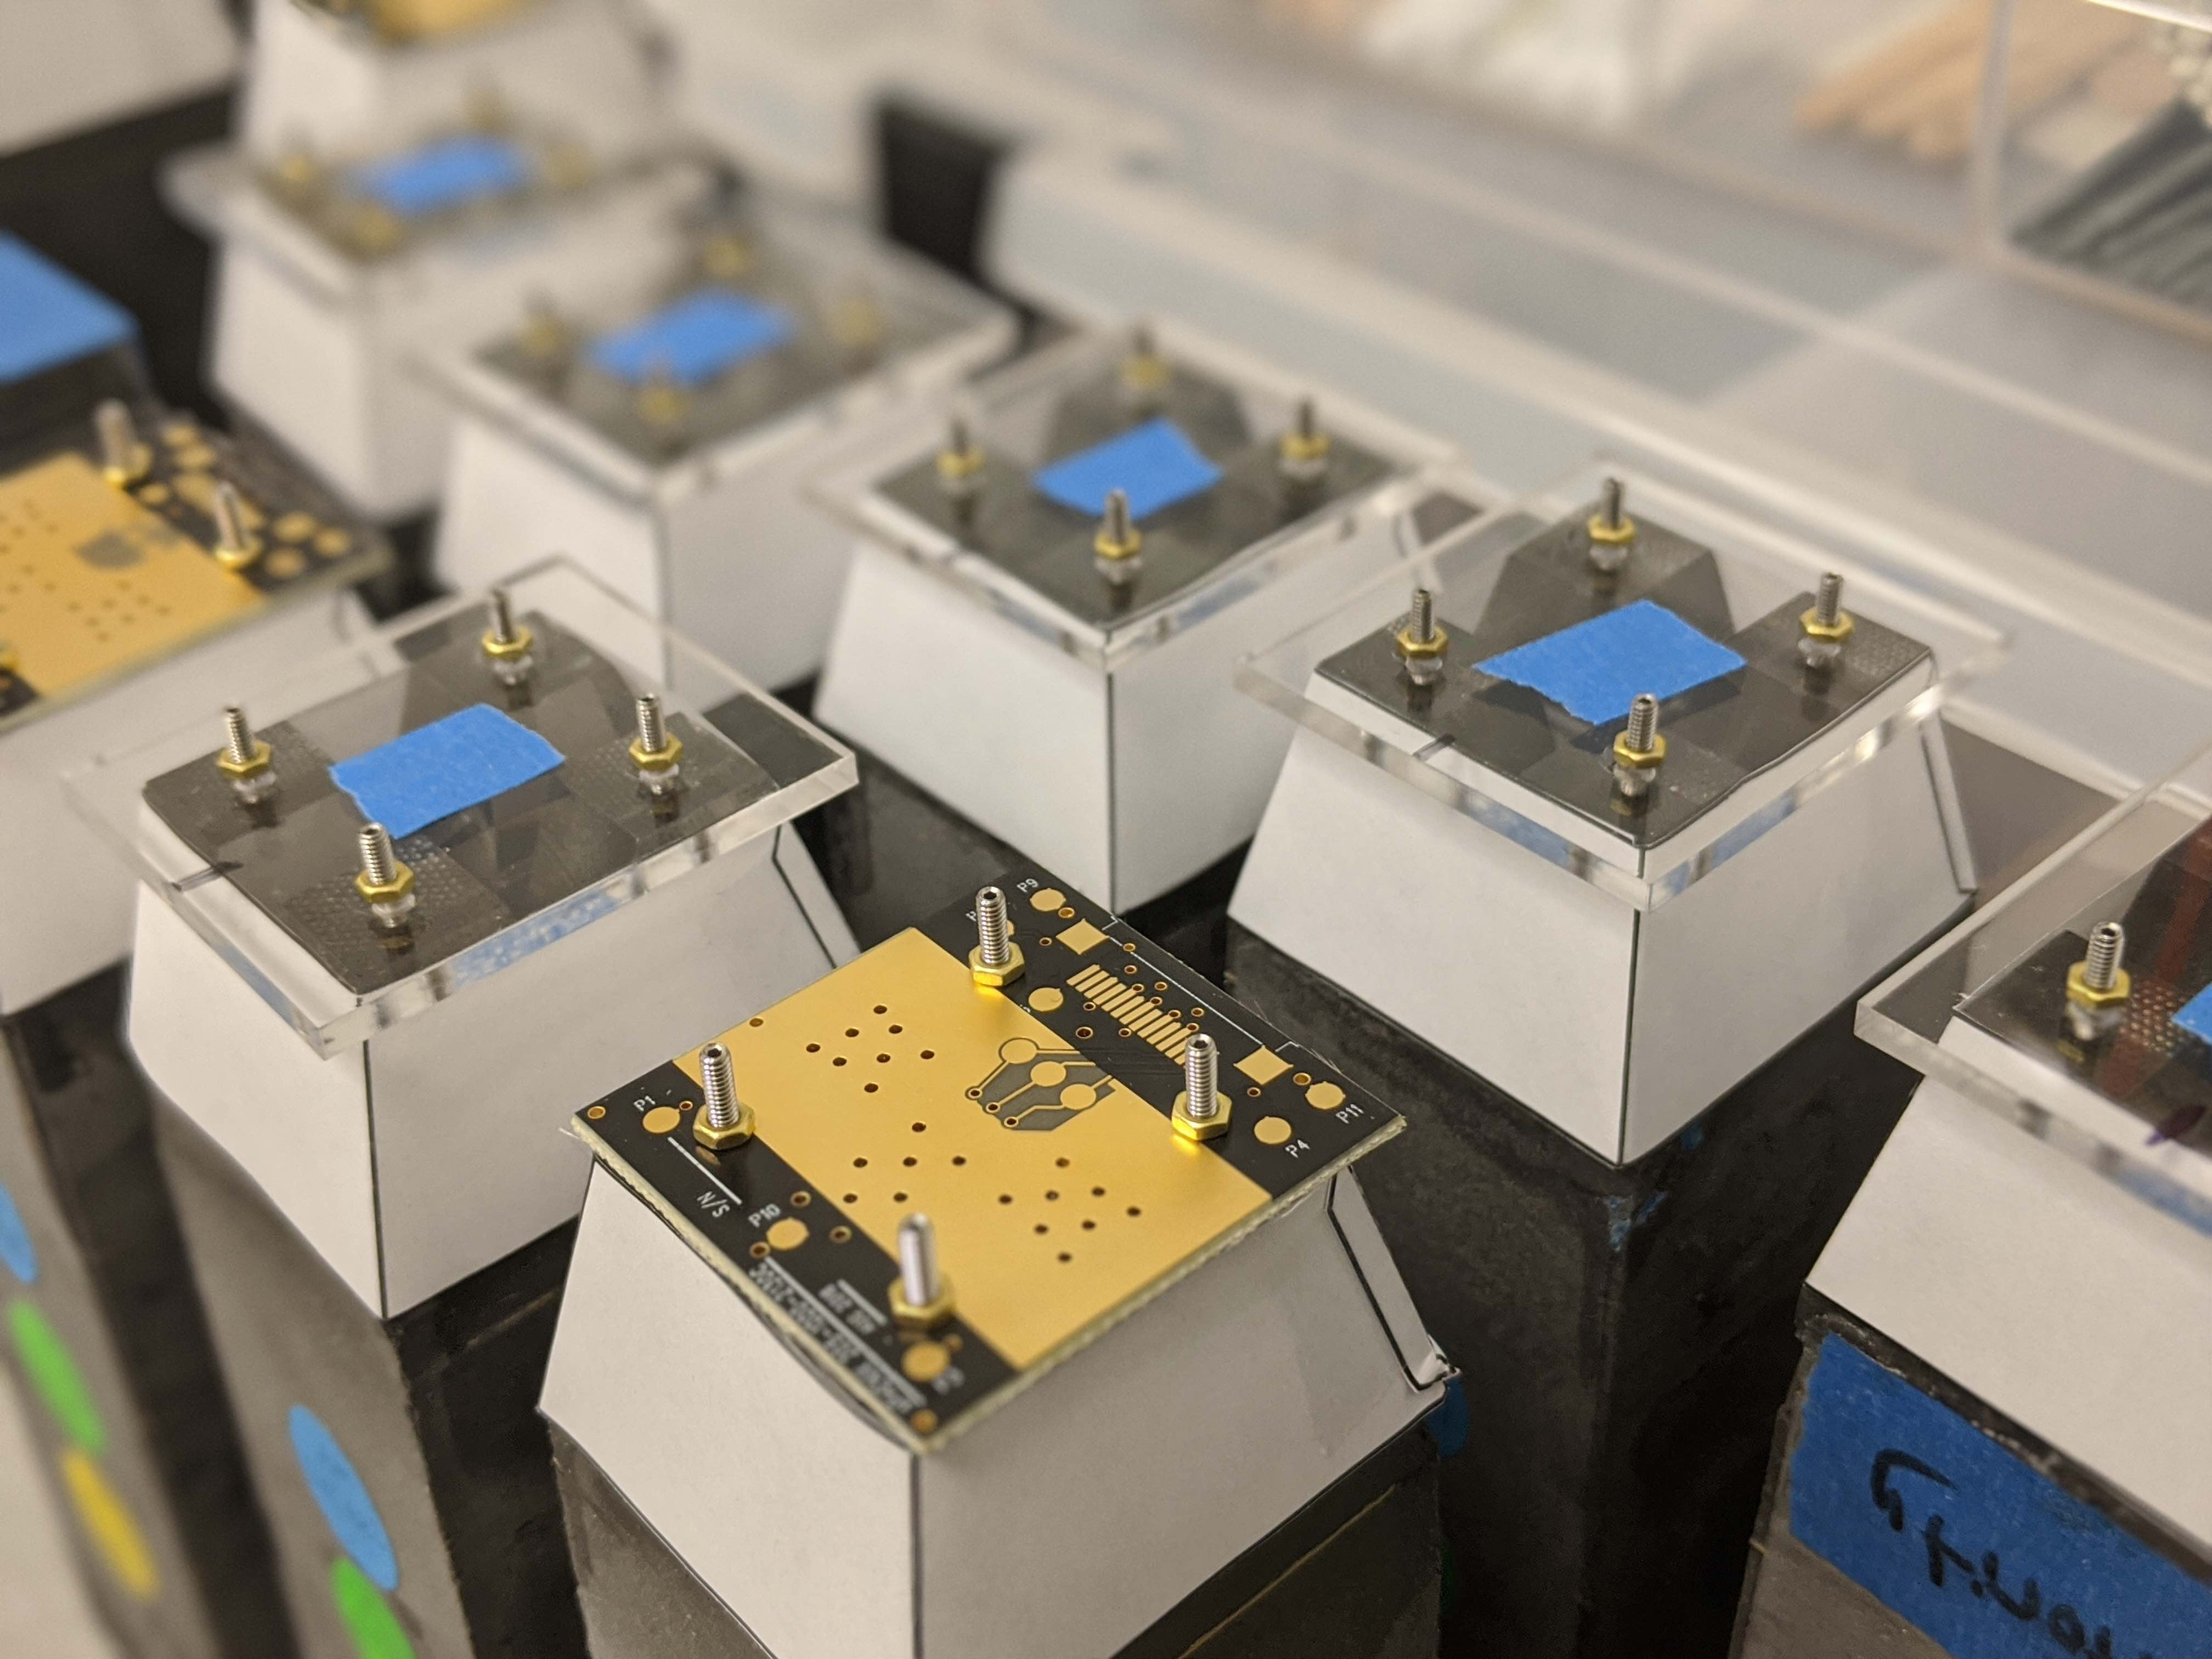
\includegraphics[trim = 0 0 1000 0, clip, width=0.62\linewidth]{emcalblocks}
  \hfill
  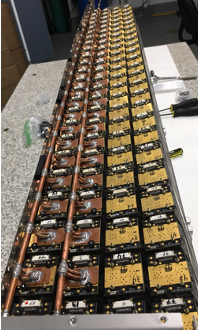
\includegraphics[width=0.37\linewidth]{sector0}
  \caption{The EMCal blocks with light guides and readout mounting (left) and the assembled EMCal Sector ``0'' (right).}
  \label{fig:emcal}
\end{figure}

\begin{figure}[hbt!]
  \centering
  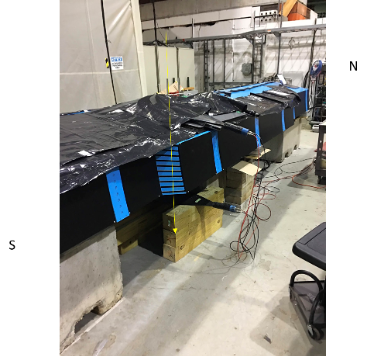
\includegraphics[trim = 20 0 20 0, clip, width=0.56\linewidth]{ohcalsector}
  \hfill
  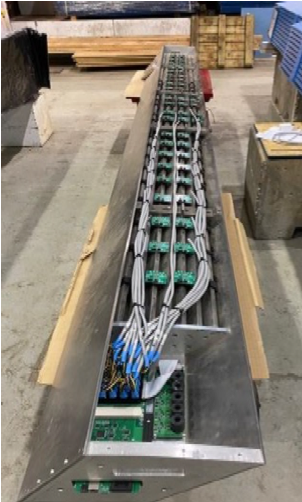
\includegraphics[width=0.42\linewidth]{ihcalsector}
  \caption{(left) Some of the outer HCal sectors being instrumented in
    Building 912 at BNL.  All 32 sectors have been delivered and are
    awaiting the installation of scintillating tiles and electronics. (right) Inner HCal sector prototype. In the final design the
    iHCal structure is made of flat aluminum plates to minimize
    costs. The iHCal is also an important support structure for all
    the detectors inside the bore of the Babar superconducting
    solenoid.}
  \label{fig:hcal}
\end{figure}

\begin{figure}[hbt!]
  \centering
  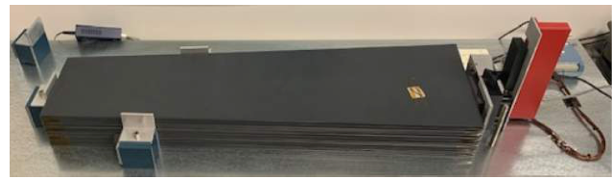
\includegraphics[width=0.75\linewidth]{tiletesting}
  \caption{Testing the HCal scintillator tiles at GSU.}
  \label{fig:tiletesting}
\end{figure}

\begin{figure}[hbt!]
  \centering
  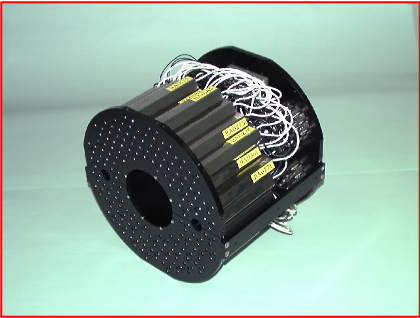
\includegraphics[trim = 5 5 5 5, clip]{mbd}
  \caption{The minimum bias detector, originally built by Hiroshima
    University for PHENIX.}
  \label{fig:mbd}
\end{figure}

The TPC inner field cage, shown in Figure \ref{fig:wagonwheel}, has been completed at SBU. The modified SAMPA ASIC (V5, with a shorter shaping time to reduce pileup effects)
has been prototyped, characterized, manufactured in quantity sufficient for the detector, and production testing is ongoing at Lund University.
About 5 of 64 sectors of EMCal are being assembled at BNL after delivery of the
calorimeter blocks from the University of Illinois Urbana-Champaign (UIUC).  Figure~\ref{fig:emcal} shows the modules with light guides and readout mounting (left) and the assembled EMCal Sector ``0'' (right).
All 32 sectors of Outer HCal steel, about 400 metric tons of steel,
have been delivered to BNL, and the scintillating tiles are being installed
in Building 912, as shown in Figure~\ref{fig:hcal} (left).
The majority of the scintillating tiles have been delivered from the vendor
and have tested both at the vendor and at Georgia State University (GSU) upon receipt, as shown in Figure \ref{fig:tiletesting}.
The calorimeter electronics is in fabrication and is keeping pace with detector
construction.
Prototype electronics for the MBD have demonstrated time resolution that exceeds the
requirements.

\subsection{Infrastructure and Facility Upgrade}

The Infrastructure and Facility Upgrade project consists of modifications to the 
1008 facility needed to support the MIE and other detectors, most importantly 
support of the former BaBar solenoid into the RHIC cryogenic and power supply
systems.  
The solenoid was tested at full field at BNL in 2018, and additional cryogenic
equipment has been designed, reviewed, and purchased.

The carriage and cradle, which support the whole detector and allow it to be 
moved into the Interaction Region and positioned on the beamline, has been designed,
reviewed, purchased, and is under construction by the vendor.
All the support systems for the detector, such as the power distribution and safety systems, and the integration and installation of the detector are designed and managed as part of this project.
Modifications to the beam pipe to simplify the installation of the MVTX detector
have been designed and reviewed by C-AD, and the procurement of the modified beam pipe 
is under way.

\subsection{Inner HCal}

The support structure of the electromagnetic calorimeter will be
instrumented with scintillating tiles similar to the tiles used in the
Outer HCal as part of the Inner HCal project.  A mock up of a sector
with the proposed organization of pre-amplifiers and cables is shown
in Figure \ref{fig:hcal} (right).

\subsection{High-Rapidity EMCal} 

The section of the barrel EMCal with $|\eta|>0.85$ was de-scoped
before CD-1/3A, however it is being restored by collaborating
institutions in China.  First articles of high-rapidity
tungsten/scintillating fiber blocks produced at Fudan University have
been shipped to UIUC and have successfully passed examination and
characterization tests.

\subsection{MVTX}

The detector nearest the collision point is the MVTX, a silicon pixel
detector closely based on the ALICE ITS inner barrel using Monolithic Active Pixel Sensors (MAPS). 
Figure~\ref{fig:mvtx_oblique} shows the design of a half barrel, designed
to clam-shell over the beam pipe.  
The MVTX is capable of 5~$\mu m$ resolution for
tracks with $p_T > 1$~GeV and enables the heavy-flavor tagged jet
and open heavy-flavor programs.  
Production of the MVTX staves is
underway at CERN, and a custom carbon fiber support structure
has been designed at MIT and LANL with engineering assistance from LBNL
Two of the production MVTX staves are shown in Figure~\ref{fig:mvtx_staves}.

\begin{figure}[hbt!]
  \centering
  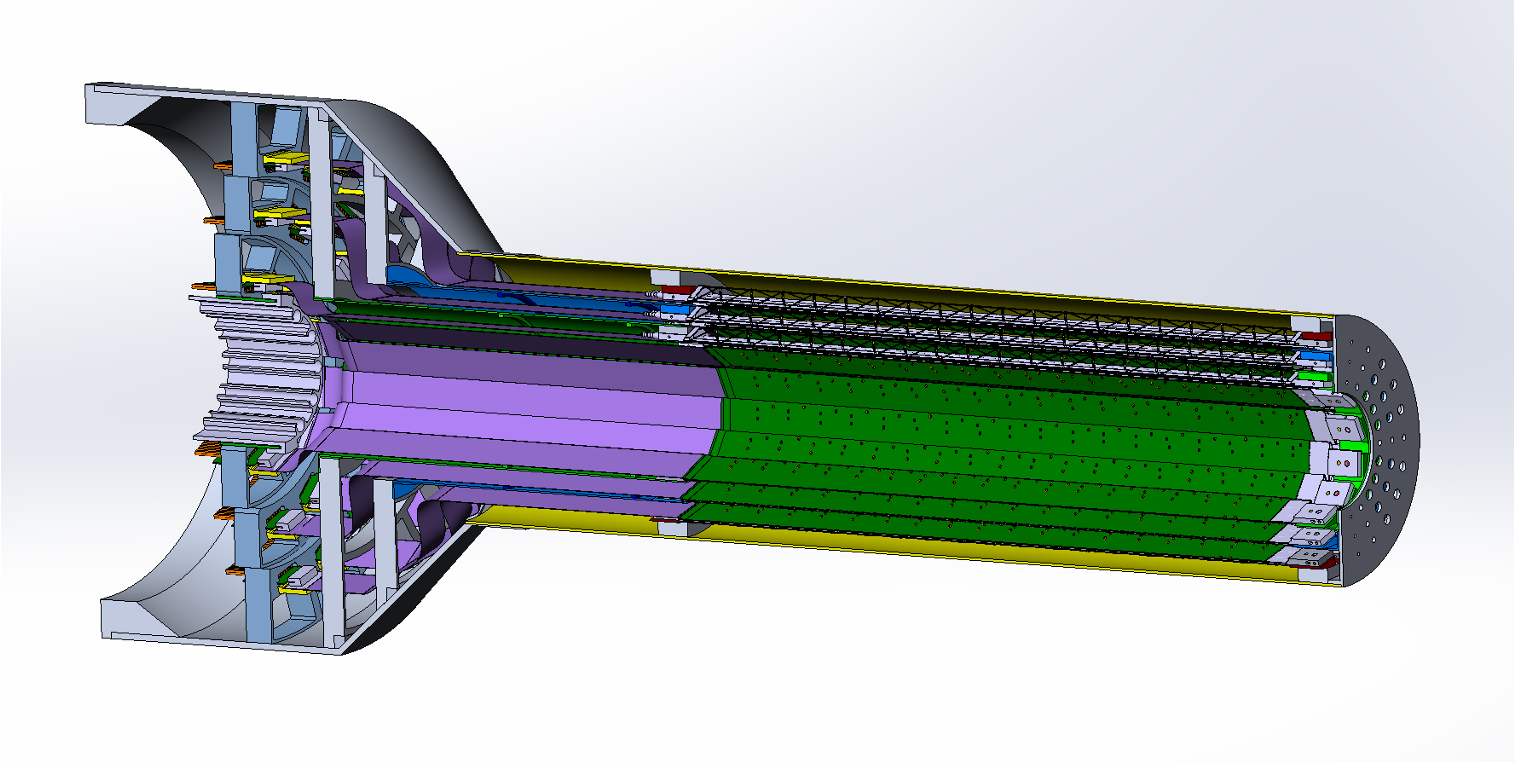
\includegraphics[width=0.9\linewidth]{mvtx_oblique}
  \caption{A rendering of a half barrel of the MVTX in its carbon
    fiber support structure.}
  \label{fig:mvtx_oblique}
\end{figure}

\begin{figure}[hbt!]
  \centering
  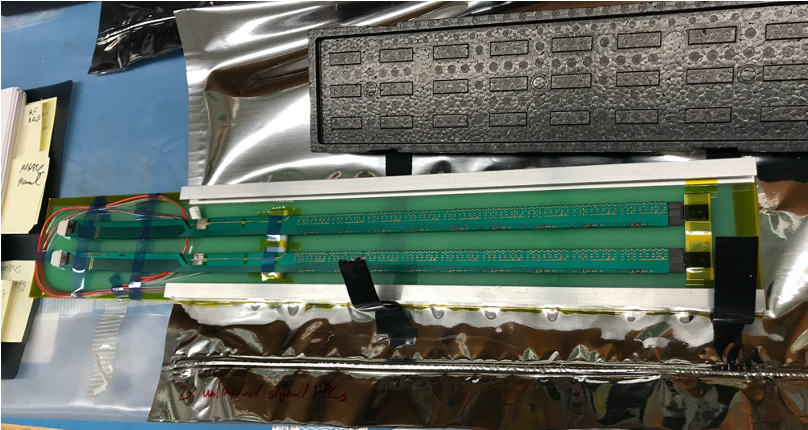
\includegraphics[width=0.9\linewidth]{mvtx_staves}
  \caption{Two of the production MVTX staves.  These are nearly
    identical to the ALICE ITS inner barrel staves.  The only
    modification is the use of a slightly longer power cable soldered
    to the stave.}
  \label{fig:mvtx_staves}
\end{figure}

\subsection{INTT}

\begin{figure}[hbt!]
  \centering
  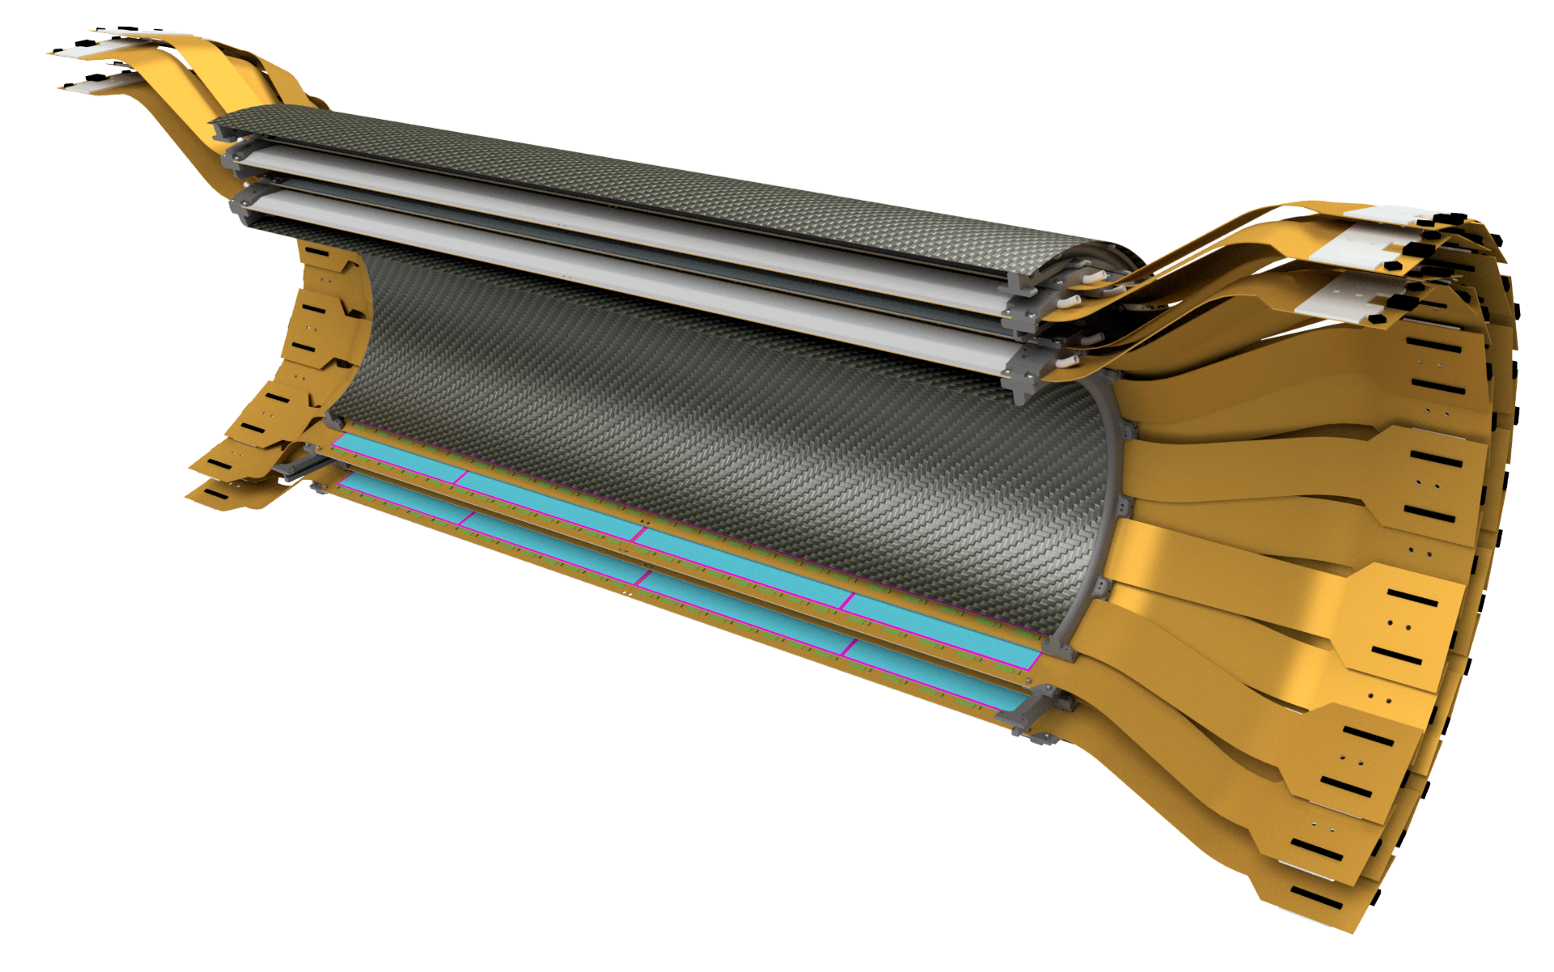
\includegraphics[width=0.77\linewidth]{intt}
  \caption{A rendering of the silicon strip intermediate tracker
    (INTT), being built by RIKEN and NCU Taiwan.  While the sensors
    (blue) are off-the-shelf Hamamatsu parts, the flexible high
    density cables (orange) which carry signals and power have been a
    target of extensive R\&D with industrial partners due to their
    length.}
  \label{fig:intt}
\end{figure}

The INTT is a silicon strip detector surrounding the MVTX, with a rendering shown in
Figure~\ref{fig:intt}.  This detector interpolates tracks between the
extremely fine pitch of the MVTX and the coarser spatial
resolution of the TPC.  It is also the only tracking detector with
single-beam-crossing timing resolution --- the ability to uniquely associate
hits with a specific bunch crossing --- and is therefore key to
associating fully reconstructed tracks with the event that produced
them.

\section{Effects of COVID-19}
\label{sec:covid}

The novel coronavirus pandemic continues to significantly affect
planning for the project.  At the same time, steps have been taken to
mitigate the most severe impacts, and these mitigations have been
largely succesful.

Project planning anticipated a large effort over the summer of 2020
coming from students and postdoctoral researcher scientists working on
the assembly and testing of detector components both at BNL and at
other labs and universities.  BNL went into a ``min safe'' mode in
late March, which halted nearly all in-person work on the oHCal and
EMCal sector assembly.  Similar stoppages happened at Fudan University
and UIUC on EMCal block production.  These efforts have recently begun
to resume, but with significant changes to work procedures.

The pandemic happened to strike at a time when major aspects of the
project could proceed remotely, and design work, reviews, and
procurements continued.  Some industries, such as steel manufacturing,
deemed essential by the US Government, continued work with little or
no interruption.

To date, the dominant effect of the pandemic on the project has been
to use up several weeks of schedule float, tightening the schedule
ahead of the early 2023 data taking.

\section{Potential relationship to EIC}
\label{sec:eic}

The potential connection between sPHENIX and the Electron Ion Collider (EIC) experimental
program has a long history.  sPHENIX traces its origin to the October
2009 charge from then ALD Steve Vigdor to the PHENIX collaboration to
detail its plans for the coming decade.  In that charge, he asked
about, ``Any plans or interest your Collaboration has in adapting your
detector or detector subsystems (or detector R\&D) to study
electron-nucleon and electron-ion collisions with an eventual eRHIC
upgrade.''  Subsequent charges from ALD Berndt Mueller have been even
more explicit in asking the potential relevance to be demonstrated
through extensive studies and documentation.  In 2013, the PHENIX
collaboration was asked to develop a ``Letter of Intent'' for an EIC
detector based on sPHENIX~\cite{Adare:2014aaa}.  In 2018, the sPHENIX collaboration was
asked to revisit this question and produce a ``design study update.''
Among the institutions that make up the sPHENIX scientific
collaboration are a significant number with acknowledged and relevant
physics expertise and interest in the EIC experimental program.  The
sPHENIX project is overseen by the ALD's office, aided by the Project
Management Committee, and sPHENIX project management has met with that
committee at least biweekly for some years, dating back to before
CD-0.  The committee membership has evolved over time but has included
experts on EIC physics and instrumentation, and they have been asked
to keep an eye on the potential reuse of parts of the sPHENIX detector
and its extensively upgraded infrastructure for a possible EIC
detector.

